\documentclass[runningheads,a4paper]{llncs}

\usepackage{verbatim}
\usepackage{amssymb}
\usepackage{amsmath} % Used for 'align' environment
\setcounter{tocdepth}{3}
\usepackage{graphicx} % Used for inserting pdf as graphics
\usepackage{float} % Used fo0r 'H' float option in figures
\usepackage{hyperref} % Used for creating a hyperlink to reference parts
\usepackage{enumitem}
\usepackage{textcomp}
\usepackage{multicol}
\usepackage{tikz}
\usetikzlibrary{positioning}
\usetikzlibrary{shapes.multipart}
\usetikzlibrary{shapes.misc} % used for rounded rectangle

\usepackage{multirow}
\usepackage{url}
\usepackage{color}
\urldef{\mailsa}\path|radelacruz@up.edu.ph|
\urldef{\mailsb}\path|fccabarle@up.edu.ph|
\urldef{\mailsc}\path|ivan.cedric10@gmail.com|
\urldef{\mailsd}\path|hnadorna@dcs.upd.edu.ph|
\urldef{\mailse}\path|zxxhust@gmail.com|
\usepackage{mathtools}
\DeclarePairedDelimiter\ceil{\lceil}{\rceil}
\DeclarePairedDelimiter\floor{\lfloor}{\rfloor}
    
\newcommand{\keywords}[1]{\par\addvspace\baselineskip
\noindent\keywordname\enspace\ignorespaces#1}
%\newcommand{\tt}[1]{\texttt{#1}}

\begin{document}


\mainmatter


\title
{
On Homogeneous Spiking Neural P System Variants
}

\titlerunning
{
Homogeneous SNPSP Systems
}


\author
{
Ren Tristan A. de la Cruz$^1$
\and
Francis George C. Cabarle$^{1,2}$
\and
Iva Cedric H. Macababayao$^{1}$
\and
Henry N. Adorna$^1$ 
\and
Xiangxiang Zeng$^3$
}

\authorrunning {de la Cruz et al}


\institute
{
$^1$Algorithms and Complexity Laboratory \\
Department of Computer Science, University of the Philippines - Diliman\\
Diliman 1101, Quezon City, Philippines    \\
$^2$Shenzhen Research Institute of Xiamen University \\
Xiamen University, Shenzhen 518000, Guangdong, China.\\
$^3$ School of Information Science and Engineering\\
Hunan University 410082, Changsha, China \\
\mailsa , \mailsb, \mailsc, \mailsd, \mailse 
}

\newcommand{\ra}{\rightarrow}

\toctitle{Lecture Notes in Computer Science}
\tocauthor{Authors' Instructions}


\maketitle

% ================================================================================================= %

\begin{abstract}

(ABSTRACT)

\keywords{Membrane Computing, 
          Spiking Neural P Systems, 
          Homogeneous Neurons,
          Structural Plasticity}
\end{abstract}

% ================================================================================================= %

\section{Introduction}

% ================================================================================================= %


\section{Spiking Neural P System and Some Variants} \label{sec-snps}

% ================================================================================================= %


\section{Homogenization of Spiking Neural P Systems} \label{sec-homo}

A \emph{state transition diagram} will be used to represent the activities of a neuron. 
A \emph{state} is a set of spike counts. For example, the set $\{4,5\}$ represents spike counts 
$4$ and $5$, the set $\{0,2,4,8,...\}$ represents even spike counts, and the set 
$\{15,20,25,30,35,...\}$ represents spike counts that are multiples of $5$ starting from $15$. 

If a neuron has $n$ spikes, the neuron is said to be \emph{in state $S$} if $n \in S$. For example, 
let $n=10$ be the number spikes in the neuron and $S_1=\{1\}$, $S_2=\{2,4,9,10,...\}$, 
$S_3=\{5,10,15,20,...\}$ be states, the neuron is not in state $S_1$ since $n \notin S_1$ but it is
in state $S_2$ and $S_3$ since $n \in S_2$ and $n \in S_3$. States can intersect since they are 
sets which means a neuron can be in multiple states at the same time. 

Most states that are associated with a given neuron represent the regular expressions of the rules
in the neuron. For example, in Figure \ref{fig-two-neurons} neuron $1$ have the rules $r_1: a/a \ra \lambda$ and  
$r_2: a(a^2)^+/a^2 \ra a$, the state $S_1=\{1\}$ represents the regular expression $a$ of rule $r_1$ 
while the state $S_2=\{3,5,7,9,11,...\}$ represents the regular expression $a(a^2)^+$ of rule $r_2$.
Neuron $1$  
 
                                                                                                
Figure \ref{fig-two-neurons}

\begin{figure}[H]                                                                                    
\begin{center}                                                                                         
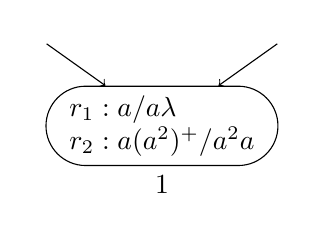
\begin{tikzpicture}                                                                                     
[                                                                                                       
neuron/.style={rounded rectangle, draw, minimum size = 10mm, align=left},                                                      
text-a/.style={black},                                                                                   
]                                                                                                       
\node (n1)   [neuron]                              {$r_1: a/a \ra \lambda$ \\ 
                                                    $r_2: a(a^2)^+/a^2 \ra a$};
\node (n1-d) [text-a, below       = 00.00mm of n1] {$1$};                                      
\node (s11)  [text-a, above right = 07.00mm of n1] {};                                      
\node (s12)  [text-a, above left  = 07.00mm of n1] {};
\draw [->]   (s11) -- (n1);                                    
\draw [->]   (s12) -- (n1);                                    
\end{tikzpicture}                                                                                       
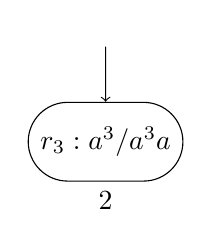
\begin{tikzpicture}                                                                                     
[                                                                                                       
neuron/.style={rounded rectangle, draw, minimum size = 10mm, align=left},                                                      
text-a/.style={black},                                                                                   
]                                                                                                       
\node (n2)   [neuron]                        {$r_3: a^3/a^3 \ra a$};
\node (n2-d) [text-a, below = 00.00mm of n2] {$2$};                                      
\node (s21)  [text-a, above = 07.00mm of n2] {};                                      
\draw [->]   (s21) -- (n2);                                    
\end{tikzpicture}                                                                                       
\end{center}
\caption{Example Neurons}                                                                                            
\label{fig-two-neurons}
\end{figure}                                                                                            

% ================================================================================================================================================== %

\bibliographystyle{splncs03}
\bibliography{homonegenous-snp}

\end{document}
